\chapter{Implementation}

\begin{markdown}
  
# Introduction #

This chapter describes the implementation of the GPU support for Julia
presented in this report. The implementation consists three
phases. __1)__ Creating a LLVM loadable module from a Julia function,
__2)__ lowering the function to code executable by a GPU and __3)__
compiling the code into ptx.

The CUDA.jl library is used as a glue to transfer data to and from the
device and schedule the generated code on the device.

# Overview #

\begin{figure}[H]
  \centering
  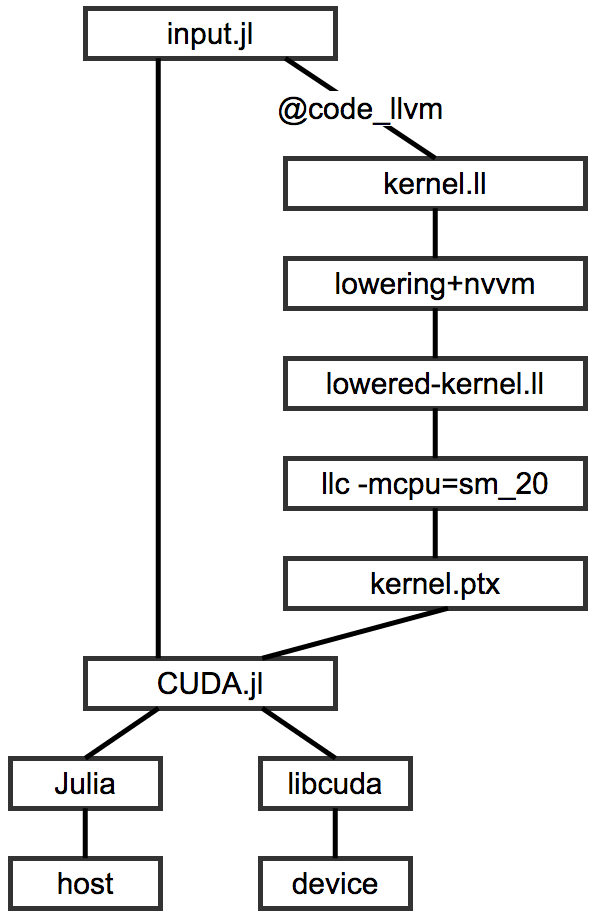
\includegraphics[width=100px]{body/figures/compiler.png}
  \caption{}
  \label{fig:compiler}
\end{figure}

In figure \ref{fig:compiler} the process of the code generation is
illustrated. A julia function is turned into LLVM IR with the compiler
builtin macro __@code\_llvm__. This code is then lowered into code
that the LLVM PTX backend can create PTX code for. Here the llc
compiler is employed directly without modification. This PTX code can
then be loaded and executed on the GPU with CUDA binding written for
Julia.


# A Guided tour through the compiler #
This section will go though the compiler step by step looking at the
generated code to show how the code is transformed. Consider the
julia kernel function in figure \ref{fig:julia-copy}. 

\begin{figure}[H]
  \begin{minted}{julia}
function copy(from, to)
  i = get_global_id(0);
  to[i] = from[i];

  return
end
  \end{minted}
  \caption{}
  \label{fig:julia-copy}
\end{figure}

## A LLVM module for Julia Function ##

The macro __@code\_llvm__ compiles a julia function with arguments
down to the corresponding LLVM IR representation. In order to load
this string into a LLVM module function declarations and types used
in the function must be included. As seen in Figure
\ref{fig:copy-llvm} the extra information need is included.

\begin{figure}[H]
  \begin{minted}{llvm}
%jl_value_t = type { %jl_value_t* }
   
define void @"julia_copy;81946"(%jl_value_t*, %jl_value_t*) {
top:
  %2 = call i64 @"julia_get_global_id;81947"(i64 0)
  %3 = call i64 @"julia_getindex;81948"(%jl_value_t* %0, i64 %2)
  %4 = call i64 @"julia_setindex!;81949"(%jl_value_t* %1, i64 %3, i64 %2)
  ret void
}

declare i64 @"julia_setindex!;81949"(%jl_value_t*, i64, i64)
declare i64 @"julia_getindex;81948"(%jl_value_t*, i64)
declare i64 @"julia_get_global_id;81947"(i64)
  \end{minted}
  \caption{}
  \label{fig:copy-llvm}
\end{figure}

The lowering LLVM pass transforms the function in figure
\ref{fig:copy_llvm} to the one in figure \ref{fig:copy_lowered}.  In
this step the gpu native implementations of for the arrays have been
linked and inlined, in place of the calls to __getindex__ and
__setindex!__ in Figure \ref{fig:copy_llvm}. The
__get_global_id__ function has been mangled to enable it to be linked
with its implementation in the next step. The julia arrays represented
with __jl_value_t__ has been replaced with a simple integer pointer in
the _global_ address space. The __!nvvm.annontations__ named metadata
is set up so the PTX backend recognizes the function as a kernel. 

\begin{figure}[H]
  \begin{minted}{llvm}
target datalayout = "e-p:32:32:32-i1:8:8-i8:8:8- ... -v1024:1024:1024"
target triple = "nvptx64-nvidia-cuda"

declare i64 @_Z13get_global_idj(i32)

define void @copy(i64 addrspace(1)*, i64 addrspace(1)*) {
top:
  %2 = call i64 @_Z13get_global_idj(i32 0)
  %3 = getelementptr inbounds i64 addrspace(1)* %0, i64 %2
  %4 = load i64 addrspace(1)* %3, align 8, !tbaa !2
  %5 = getelementptr inbounds i64 addrspace(1)* %1, i64 %2
  store i64 %4, i64 addrspace(1)* %5, align 8, !tbaa !2
  ret void
}

!llvm.ident = !{!0}
!nvvm.annotations = !{!1}

!0 = metadata !{metadata !"Apple LLVM version 6.0 (clang-600.0.54) (based on LLVM 3.5svn)"}
!1 = metadata !{void (i64 addrspace(1)*, i64 addrspace(1)*)* @copy, metadata !"kernel", i32 1}
  \end{minted}
  \caption{}
  \label{fig:julia-copy}
\end{figure}

\end{markdown}
